\chapter{Organisation}
Dette afsnit vil give et indblik i strukturen og opbygningen af Kvindeafdelingen, Svangre- og ultralydsambulatorium på Hospitalsenheden Horsens (HEH) og afdeling Kvindesygdomme og Fødsler på Regionshospitalet Midt Viborg (RMV). Afsnittet vil belyse, hvilken betydning implementeringen af en Ultralyds Robotarm, vil have for afdelingerne som organisation, samt hvilke ændringer dette vil medføre i arbejdsgangen for personalet. \\
Informationer, som er indhentet fra HEH og RMV, vil blive sammenholdt med videnskabelige artikler, i forsøget på at finde en større sammenhæng i problemstillingen omkring arbejdsgener ved ultralydsscanning. 

Det er valgt, at benyttes Leavitts organisationsmodel \ref{DiamantModel} som analysemetode. Denne model er en diamantmodel, der arbejder med fire organisatoriske hovedelementer, der relaterer sig til hinanden. Hvert hovedelement vil blive belyst i hvert sit underafsnit. \cite{Leavitt} \cite{diamantmodel} 

\begin{figure}[h!]\centering
	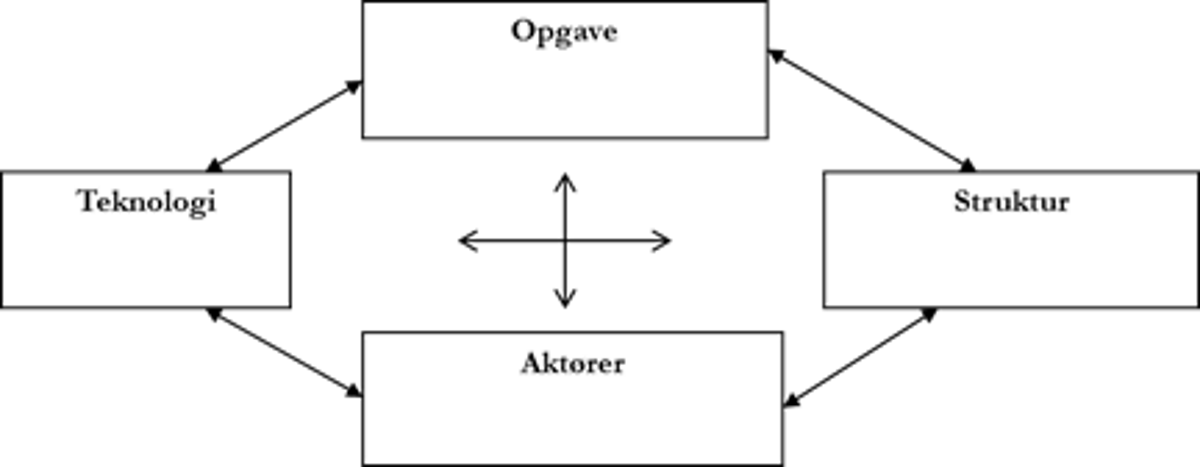
\includegraphics[width = 0.7\textwidth]{Figurer/LeavittModel}
	\caption{Leavitts organisationsmodel, viser hvordan struktur, aktører, opgaver og teknologi indbyrdes relaterer sig til hinanden, i midten haves kulturen for organisationen. \cite{diamantmodel}}
	\label{DiamantModel}
\end{figure}

Da analysen kun bygger på dataindsamling fra to kliniske afdelinger på HEH og RMV, vil dens generaliserbarhed potentielt være begrænset. Resultatet heraf kan derfor ikke nødvendigvis anvendes på samtlige lignende hospitalsafdelinger i Danmark. 

Dataindsamlingen til analyse er indhentet gennem interview med afdelingssygeplejerske Tina Arnbjørn og tre sonografer fra HEH, samt interview med afdelingssygeplejerske Karen Marie Goul og en sonograf fra RMV.
Til at underbygge arbejdsskadeproblemstillingen benyttes yderligere videnskabelige artikler.

\section{HEH}
HEH er bemandet af en afdelingssygeplejerske, fem sonografer samt et ukendt antal læger. Antallet af læger er ikke relevant for denne analyse, da der udelukkende fokuseres på sonografernes arbejdsgange.
Afdelingen har udstyr til fire stuer, hvoraf tre stuer bemandes af sonografer. Der foretages 30-40 scanninger om dagen på afdelingen, hver scanning tager i gennemsnit 35 minutter. 
Ovenstående information er blevet opsamlet under interview med afdelingssygeplejerske Tina Arnbjørn på HEH. (se Bilag 4)

\section{RMV}
Bemanding på RMV består af en afdelingssygeplejerske, ni sonografer og et ukendt antal læger. Afdelingen har ultralydsscanningsudstyr til fem stuer til gravide, hvoraf tre stuer er i drift dagligt og bemandes af sonografer. Dagligt foretages der 25-30 scanninger på afdelingen. En scanning tager i gennemsnittet 30 minutter.
Informationerne for RMV er opnået igennem interview med afdelingssygeplejerske Karen Marie Goul. (se Bilag 5)

\section{Leavitts organisationsmodel}
Det er valgt at sammenskrive de indsamlede data fra HEH og RMV, da afdelingerne på de to hospitaler er sammenlignelige. Leavitts organisationsmodel er med til at give et billede af de to afdelingers organisation og struktur. Derudover vil modellen belyse, hvordan organisationsstrukturen, opgaver og organisationens ansatte bliver påvirket af implementeringen af den nye teknologi. \cite{Leavitt} \cite{diamantmodel} 


\subsection{Opgaver}
Opgaverne som afdelingerne varetager på nuværende tidspunkt, vil ikke ændre sig ved implementering af robotarmen. Dette skyldes at behovet for scanninger af gravide forbliver uændret. Opgaverne består af nakkefoldsscanning i 11.-13. uge, misdannelsesscanning i 19.-22. uge, vægtscanninger samt andre kontrolscanninger i løbet af graviditeten. \cite{graviditet} 

\subsection{Teknologi}
Ved implementering af en ny teknologi, som Ultralyds Robotarmen, vil det sætte krav til aktørernes faglige kundskaber og erfaringer i brugen af teknologien. Dette er gældende for samtlige sonografer der skal benytte Robotarmen. Derfor skal der være en indkørselsperiode af teknologien førend, at den vil være i fuld brug og alt personale har den rette kendskab i brugen af robotarmen. \\
Det vurderes, at de eksisterende stuer på HEH og RMV er tilstrækkelig store til at teknologien vil kunne implementeres uden yderligere ændringer. På RMV kan det dog blive nødvendigt at flytte patientskærmen, da robotarmsstativet muligvis vil komme til at dække for den gravides udsyn til skærmen.  

\subsection{Aktører} \label{aktoerer_organisation}
Muskel- eller skeletbesvær forårsaget eller forværret af de arbejdsopgaver, som udføres på arbejdspladsen er work-related musculoskeletal disorders (WRMSD). De fremkommer ved gentagne belastninger, kraftkrævende eller akavede bevægelser. I 2008 oplevede 90\% af sonograferne smerter under udførelsen af scanninger. Disse smerter kan blive en økonomisk og personlig udgift for sonograferne.\cite{31}\cite{30}\\
Billedet af at 90\% af sonograferne mærker til smerter under scanninger blev også gjort klart på både HEH og RMV, hvor udtalelser fra sonograferne underbyggede netop dette. Her er den udbredte mening, at arbejdet er belastende og der derfor er usikkerhed om hvor længe de kan blive i stillingen. Det belastende arbejde, sammen med den stigende tendens for de gravides BMI, skaber grund til denne usikkerhed. \cite{kvinderovervaegt} \\
Dog er sonograferne positive omkring deres stilling, hvilket også kan være med til at undertrykke smerterne, sådan at sonografen kan forblive i sin stillingen.

Disse skader og smerter ses i nakke, skulder og håndled og kan forekomme af drejende bevægelser i nakke og krop, håndledsbøjninger og arbejde i udstrakt arm. Smerterne kan også stamme fra inflammation af senerne i hånd og håndled, hvilken forekommer af belastningen fra grebet om ultralydsproben sammen med håndledsbøjninger \cite{31}. Se figur \ref{wrist} og \ref{udstraktArm}.

\begin{figure}[H]
  \begin{minipage}{0.49\textwidth}
    \centering
      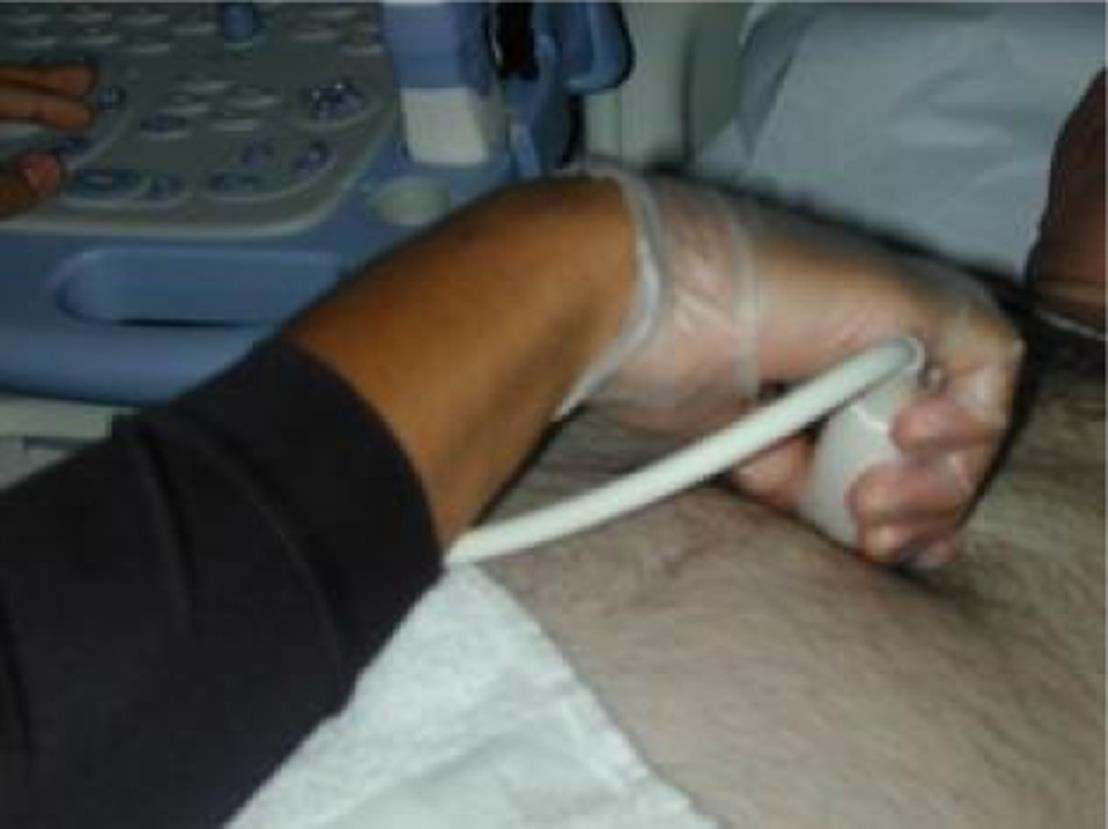
\includegraphics[width=\textwidth]{Figurer/wrist.jpg}
      \caption{Håndledsbøjning og greb om proben \cite{31}}
    \label{wrist}
  \end{minipage}
  \hspace{0.02\textwidth}
  \begin{minipage}{0.47\textwidth}
    \centering
      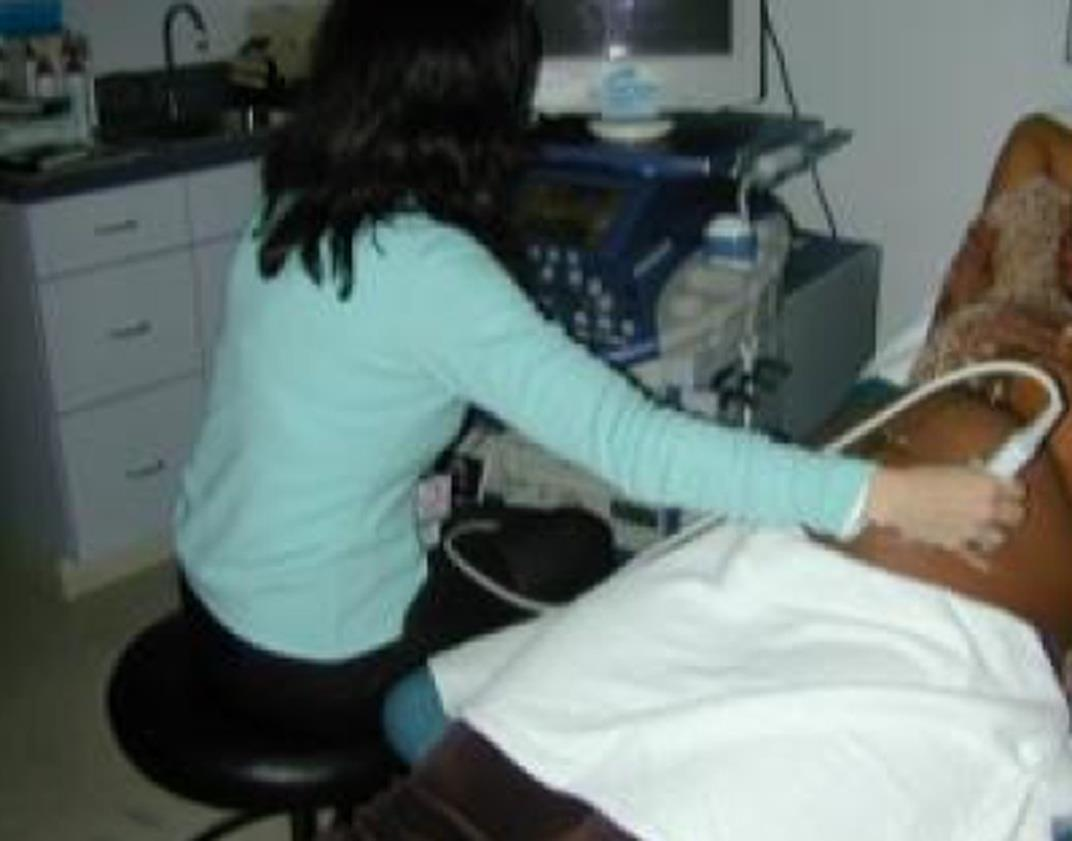
\includegraphics[width=\textwidth]{Figurer/arm.jpg}
      \caption{Arbejde i udstrakt arm \cite{31}}
    \label{udstraktArm}
  \end{minipage}
\end{figure}

Implementeringen af robotarmen vil føre til markante ændringer for sonografernes arbejdsstillinger. Disse ændringer sker, idet sonografen ikke længere skal sidde med strakt arm ind over den gravide, og skaderne i skulderen vil derfor kunne undgås. Desuden vil sonografen være mere centreret omkring arbejdsstationen og derfor vil vrid i kroppen og nakken også blive mindsket. Sonografen skal dog stadig holde om dummy-proben, se under kapitel \ref{Teknologi}, så den gribende belastning kan ikke fjernes helt. Men sammen med at de resterende belastninger kan mindskes eller helt fjernes, vil dette ikke have den samme belastende virkning. 

En undersøgelse er blevet udført af Robotic Ultrasound for at tjekke, hvor mange kilo sonograferne skal påtrykke proben med under ultralydsscanningerne. Her blev proben påført en dynamometer, hvilken skulle måle trykket som sonografen skulle påtrykke med under scanning. Resultatet heraf blev at sonograferne ved de almindelige og ukomplicerede scanninger, som ved en nakkefoldsscanning, trykker med 2-3 kg, hvor sonograferne skal trykke med omkring 11 kg ved de mere komplicerede scanninger, som scanning på gravide med bagoverbøjet livmoder. Trykket føles dog større for sonografen, da dette arbejde og dermed trykket skal påføres i udstrakt arm. Undersøgelsen blev kun udført på 5 sonografer over én arbejdsdag. (se Bilag 12, 28.04.2016)

Den generelle holdning på HEH og RMV er meget teknologivenlig. Derfor formodes det, at implementeringen af teknologien ikke vil føre til væsentlige problemer i forhold til at få sonograferne til at benytte Ultralyds Robotarmen. Implementeringen kræver dog, at der tilrettelægges en ordentlig plan for oplæring af sonograferne i brugen af teknologien. Sonograferne har generelt en god holdning og tillid til teknologi og er åbne for en mulig implementering af Ultralyds Robotarmen.

\subsection{Struktur}
Pr. juni 2016 er den strukturelle opbygning på afdelingerne således, at en medarbejder ultralydsscanner henholdsvis 30 timer på HEH og 22 timer på RMV om ugen. De resterende timer udmønter sig som aflastende arbejde for den enkelte medarbejder. Denne struktur skyldes, at det er et kendt problem på afdelingerne, at scanningsarbejdet er fysisk belastende for medarbejderen. I løbet af en scanningsdag har én medarbejder i gennemsnit ti scanninger. Yderligere foretages der på afdelingerne forebyggende tiltag, i form af styrketrænende delastikøvelser, mulighed for gratis massage, ergonomiske redskaber samt fri adgang til fysioterapeuter og wellness-konsulenter, der kontrollerer og vejleder om medarbejderens arbejdsstillinger. (se Bilag 4 og Bilag 5)

Afdelingerne tilrettelægger selv mængden af tid den enkelte sonograf skal scanne i løbet af en uge. Men Dansk Føtalmedicinsk Selskab udstikker hvert femte år anbefalinger, som det anbefales afdelingerne at følge. Anbefalingerne i forhold til antal timers ultralydscanning er 28 timer pr. uge, da det er vurderet at ved denne mængde af scanninger vil belastningen af sonografen ikke være i en skadende grad (Se Bilag 10). Denne vurdering underbygges af videnskabelige forskningsundersøgelser, hvor sonografernes arbejdsskader og mængden af scanningstid er blevet sammenholdt. Disse undersøgelser viser yderligere at en arbejdsskade typisk først optræder efter 5 år, hvilket der skal tages højde for i valget af observationsgruppe til lignende undersøgelser \cite{35}.

Ud fra dette bemærkes det, at RMV arbejder 6 timer under anbefalingerne, mens sonograferne på HEH scanner to timer mere om ugen end anbefalet. Årsagerne hertil kan være flere. Typisk vil grunden til dette være at normeringerne og bevillingerne til antal af sonografer og antallet af scanninger, der skal udføres, ikke gør det muligt at tilpasse arbejdsforholdet til anbefalingerne. 

Implementering af robotarmen vil føre til en ændring i afdelingernes strukturelle opbygning. Ultralyds Robotarmen vil gøre scanningsarbejdet væsentlig mindre belastende, og dermed vil det kunne føre til at en medarbejder vil kunne scanne på fuldtidsbasis, altså 37 timer om ugen. Arbejdsstillingerne som sonograferne udfører og hvordan disse vil ændre sig, er beskrevet i afsnittet \ref{aktoerer_organisation}. Hvis sonograferne scanner 37 timer om ugen, vil de opgaver som sonograferne varetager som aflastende arbejde, herunder bl.a. fostervandsprøver (se Bilag 4) og medicinske aborter (se Bilag 5), kunne blive varetaget af andet personale. Yderligere kan det føre til en ændring i antallet af sonografer, der er behov for på den enkelte afdeling. 

HEH har på nuværende tidspunkt indvilliget i at være testafdeling for Robotic Ultrasound ApS under udviklingen og test af produktet. Det er i afdelingens interesse, da der ses en fremtid i produktet. Det ønskes fra afdelingens side at være med under tilpasningen af produktet til afdelingens struktur og behov. 

\section{Delkonklusion}


